\documentclass[conference]{IEEEtran}

\usepackage{url}
\usepackage{graphicx}
\usepackage{caption}
%\usepackage{subcaption}
\usepackage{subfigure}
\usepackage{hyperref}
\usepackage{url}
\usepackage{times}
\usepackage{balance}
\usepackage{xspace}
\usepackage{paralist}
\usepackage{color}
\usepackage{amssymb}

\clubpenalty = 10000
\widowpenalty = 10000
\displaywidowpenalty = 10000

\begin{document}

\newcommand{\ghtorrent}{\textsc{ght}orrent\xspace}
\newcommand{\prioritizer}{\textsc{pr}ioritizer\xspace}
\newcommand{\api}{\textsc{api}\xspace}
\newcommand{\todo}[1]{\textcolor{red}{\textbf{\textsc{todo:}} #1}}

\newcommand{\nb}[3]{
  \fcolorbox{black}{#2}{\bfseries\sffamily\scriptsize#1}
    {\sf\small$\blacktriangleright$\textit{#3}$\blacktriangleleft$}
}

\newcommand\georgios[1]{\nb{Georgios}{yellow}{#1}}
\newcommand\andy[1]{\nb{Andy}{cyan}{#1}}
\newcommand\erik[1]{\nb{Erik}{magenta}{#1}}

\newcommand{\hassanbox}[1]
{
  \vspace{0.29em}
  \noindent
  \fbox{
  \begin{minipage}{0.46\textwidth}
    \emph{\noindent #1}
    \end{minipage}
}}

% Macros for qualitative research :-)
\newcommand{\resp}[2]{{\sc R#1:} ``\emph{#2}''}
\newcommand{\respnum}[1]{{\sc R#1}}
\newcommand{\code}[1]{{\textsl{#1}}}

%\title{Pull Request Prioritization}
\title{Automatically Prioritizing Pull Requests}

\author{\IEEEauthorblockN{Erik van der Veen, Georgios Gousios, Andy Zaidman}
\IEEEauthorblockA{Delft University of Technology,\\The Netherlands}
\IEEEauthorblockA{\{e.v.d.veen@tudelft.nl, g.gousios, a.e.zaidman\}@tudelft.nl}
}


\author{\IEEEauthorblockN{Erik van der Veen}
\IEEEauthorblockA{Delft University of Technology\\
the Netherlands\\
Email: e.v.d.veen@tudelft.nl}
\and
\IEEEauthorblockN{Georgios Gousios}
\IEEEauthorblockA{Radboud University Nijmegen\\
the Netherlands\\
Email:georgios@cs.ru.nl}
\and
\IEEEauthorblockN{Andy Zaidman}
\IEEEauthorblockA{Delft University of Technology\\
the Netherlands\\
Email: a.e.zaidman@tudelft.nl}}

\maketitle

\begin{abstract}

In previous work, we observed that in the pull-based development model integrators face challenges with regard to prioritizing work in the face of multiple concurrent pull requests. We present the design and initial implementation of a prototype pull request prioritisation tool called \prioritizer. \prioritizer works like a priority inbox for pull requests, recommending the top 3 pull requests the project owner should focus on. A preliminary user study showed that \prioritizer provides functionality that GitHub is currently lacking, even though users needed more insight into how the priority ranking is established to make \prioritizer really useful.

\end{abstract}

%\category{D.2.7}{Software Engineering}{Distribution, Maintenance, and Enhancement}[Version control]
%\category{D.2.9}{Software Engineering}{Management}[Programming teams]

%\terms{Management}

%\keywords{pull-based development, pull request, distributed software development,
%empirical software engineering}

\section{Introduction}

Pull-based development as a distributed development model is a distinct way of
collaborating in software development. In this model, the project's main
repository is not shared among potential contributors; instead, contributors
fork (clone) the repository and make their changes independent of each other.
When a set of changes is ready to be submitted to the main repository, they
create a pull request, which specifies a local branch to be merged with a branch
in the main repository. A member of the project's core team (the
\emph{integrator}) is responsible to inspect the changes and integrate them into
the project's main development line.

In earlier work~\cite{GZSD15}, we surveyed 750 pull request integrators from high
volume projects and discovered that the top two challenges they face when
working with pull requests are maintaining project quality and prioritizing work
in the face of multiple concurrent pull requests. With respect to pull request
prioritization our findings are summarized in Figure~\ref{fig:prioritization}.

In this paper, we present the design and initial implementation of a prototype
pull request prioritization tool, the \prioritizer. \prioritizer works as a
priority inbox for pull requests: it examines all open pull requests and
presents project integrators the top 5 pull requests that need their immediate
attention. It also offers an alternative view to Github's pull request
interface, which allows developers to sort open pull requests on a multitude of
criteria, ranging from the pull request's age to its number of pairwise
conflicts. \prioritizer is a service-oriented architecture build on top of
\ghtorrent~\cite{G13}: it uses \ghtorrent's data collection mechanisms to react in near
real-time to changes in pull request state \andy{I would drop 2nd part of sentence} and databases as a source of easy to
access metadata.


\begin{figure}[t]
  \begin{center}
    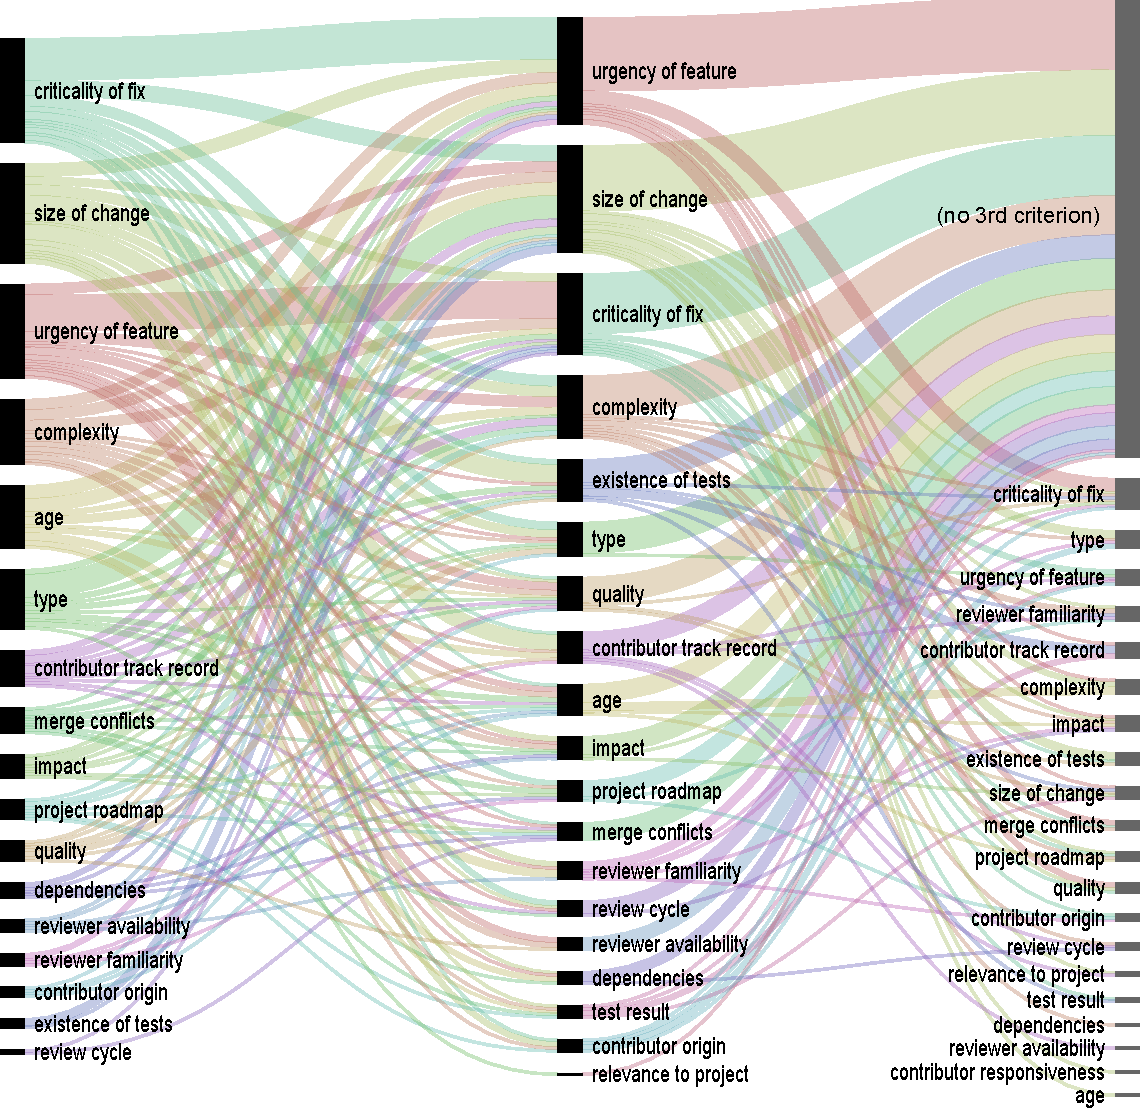
\includegraphics[scale=0.44]{prioritization-criteria}
    \andy{Figure is currently missing. Forgot to commit?}
  \end{center}
  \caption{Prioritization criteria and their order of application as reported by
  750 integrators.}
  \label{fig:prioritization}
\end{figure}


\section{Prioritizing pull requests}

\subsection{Modeling} Contrary to common approaches to work prioritization, which usually produce
an optimal ordering for open work items based on optimization processes, we
modelled the pull request prioritization using the priority inbox approach~\cite{Conway2011}.
What \prioritizer tries to do is present the integrators with the 3 pull
requests that will need their immediate attention. \andy{Need some related
work support here}

To select the important pull requests, \prioritizer uses machine learning.
Initially, time is split in configurable time windows (currently, 1 day long).
In each time window, it calculates a list of features for all pull requests
(dependent variables, explained below) and a boolean response variable that
indicates whether the received a user action in the following time window. A
machine learning algorithm is then applied on historical data to build a model
for predicting whether current pull requests will receive user updates in the
following time window. The 3 pull requests with the highest probability to be
updated are classified as the important ones.

\subsection{Features}
\label{sec:features}
Our feature set was extracted by analysing the results of the survey~\cite{GZSD15} and
closely correspond to the developer's answers are reported in
Figure~\ref{fig:prioritization}. An overview of the selected features can
be seen in Table~\ref{tab:features}.

\begin{table*}[ht]
  \centering
  \begin{tabular}{rp{26em}rrrrc}
    \hline
    \textbf{Feature} & \textbf{Description} & \textbf{5\%} & \textbf{Mean} & \textbf{Median} & \textbf{95\%} & \textbf{Plot} \\
    \hline
    Age & Minutes between open and the current time window start time. & 0.00 & 167344.02 & 77760.00 & 646560.00 & 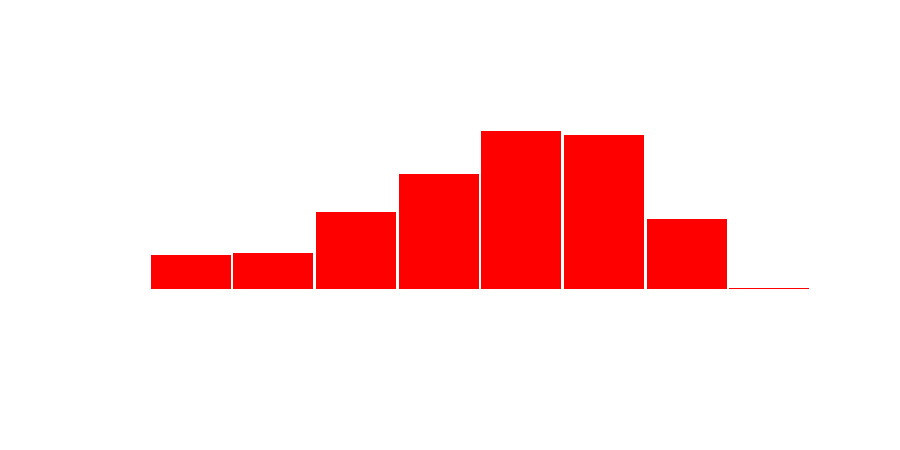
\includegraphics[scale = 0.1, clip = true, trim= 50px 60px 50px 60px]{../figs/hist-features/hist-age.pdf} \\
    Contribution Rate & The percentage of commits by the author currently in the project. & 0.00 & 0.03 & 0.00 & 0.14 & 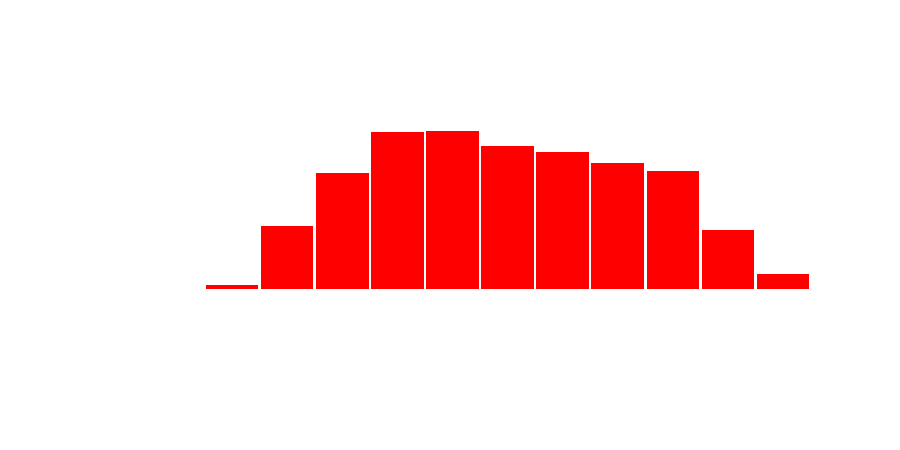
\includegraphics[scale = 0.1, clip = true, trim= 50px 60px 50px 60px]{../figs/hist-features/hist-commitRatio.pdf} \\
    Accept Rate & The percentage of the author's other PRs that have been merged. & 0.00 & 0.45 & 0.50 & 0.90 & 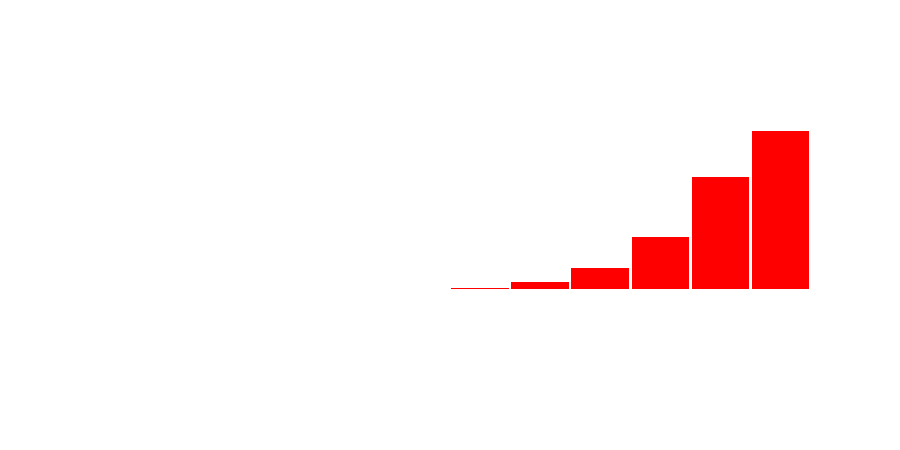
\includegraphics[scale = 0.1, clip = true, trim= 50px 60px 50px 60px]{../figs/hist-features/hist-pullRequestRatio.pdf} \\
    Additions & Number of lines added. & 1.00 & 3649.86 & 41.00 & 6285.00 & 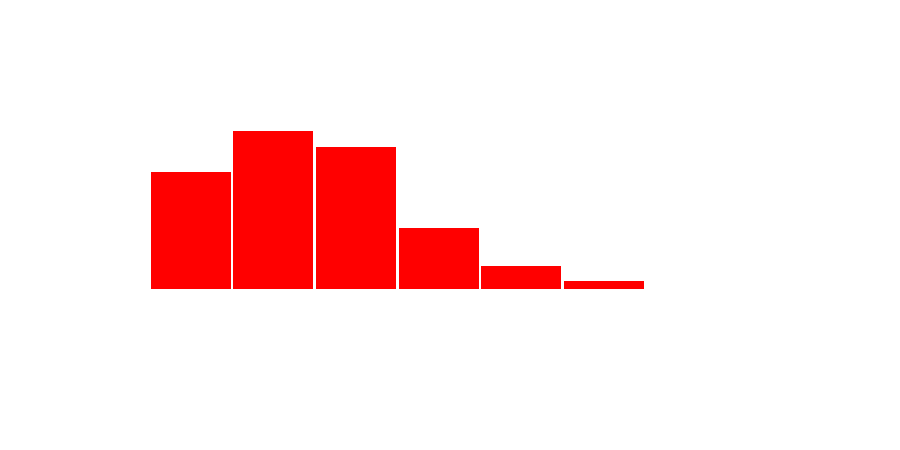
\includegraphics[scale = 0.1, clip = true, trim= 50px 60px 50px 60px]{../figs/hist-features/hist-additions.pdf} \\
    Deletions & Number of lines deleted. & 0.00 & 2271.32 & 7.00 & 2353.00 & 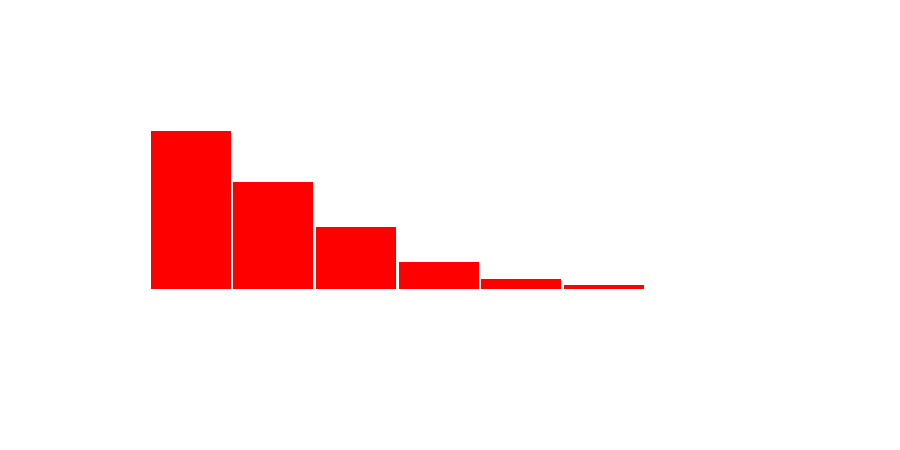
\includegraphics[scale = 0.1, clip = true, trim= 50px 60px 50px 60px]{../figs/hist-features/hist-deletions.pdf} \\
    Commits & Number of commits. & 1.00 & 6.52 & 2.00 & 22.00 & 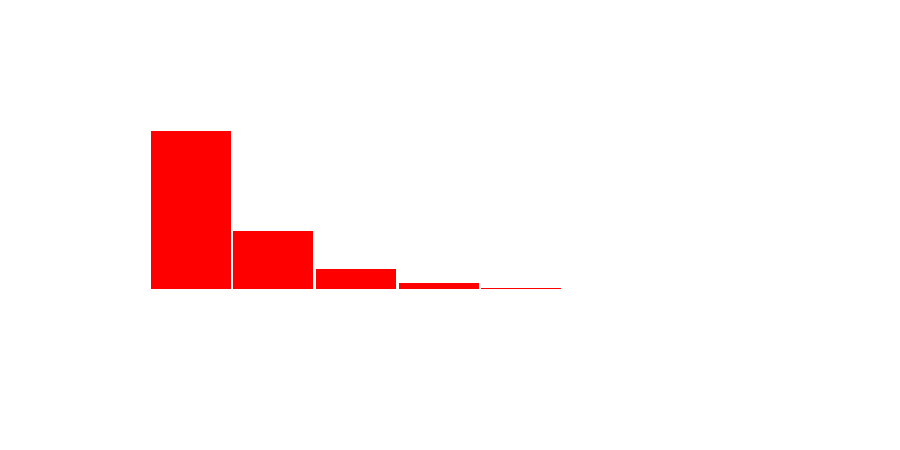
\includegraphics[scale = 0.1, clip = true, trim= 50px 60px 50px 60px]{../figs/hist-features/hist-commits.pdf} \\
    Files & Number of files touched. & 1.00 & 53.88 & 2.00 & 125.00 & 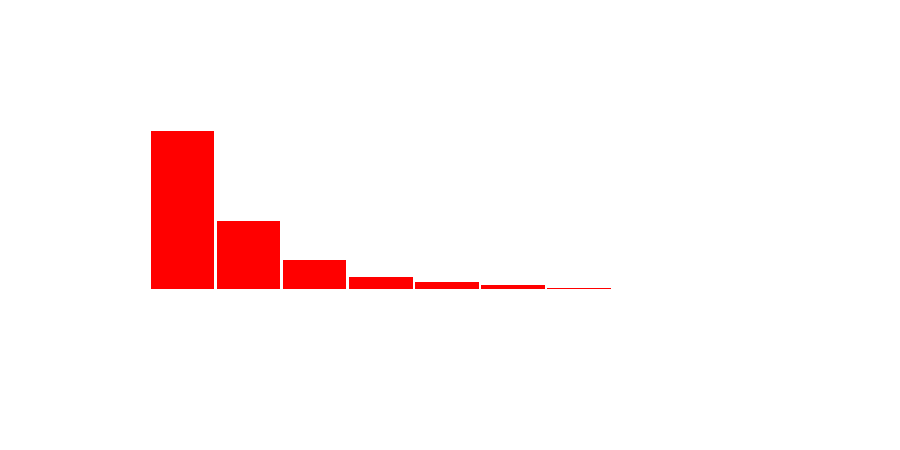
\includegraphics[scale = 0.1, clip = true, trim= 50px 60px 50px 60px]{../figs/hist-features/hist-files.pdf} \\
    Comments & Number of discussion comments. & 0.00 & 4.22 & 1.00 & 17.00 & 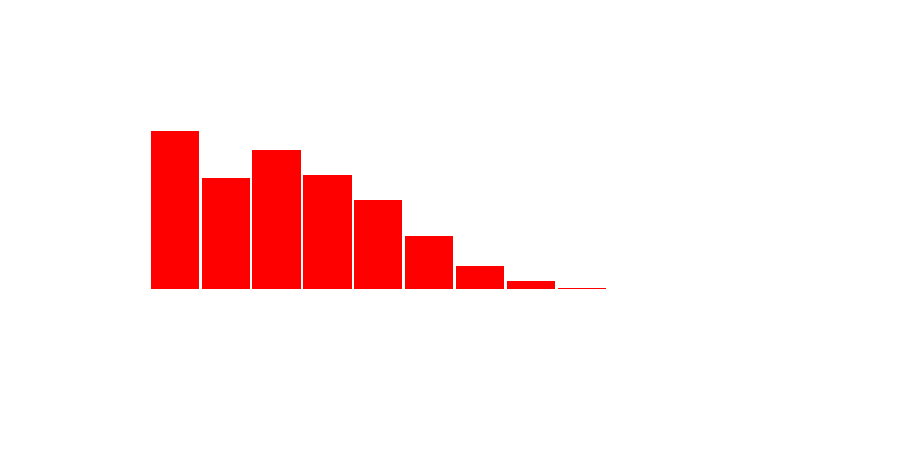
\includegraphics[scale = 0.1, clip = true, trim= 50px 60px 50px 60px]{../figs/hist-features/hist-comments.pdf} \\
    Review Comments & Number of code review comments. & 0.00 & 1.60 & 0.00 & 8.00 & 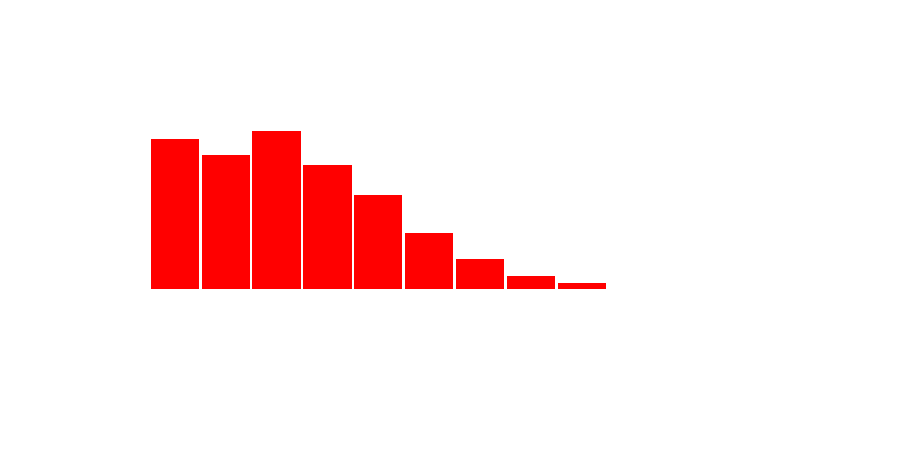
\includegraphics[scale = 0.1, clip = true, trim= 50px 60px 50px 60px]{../figs/hist-features/hist-reviewComments.pdf} \\
    Core Member & Is the author a project member? & 0.00 & 0.26 & 0.00 & 1.00 & 
\includegraphics[scale = 0.1, clip = true, trim= 50px 60px 50px 60px]{../figs/hist-features/hist-coreMember.pdf} \\
    Intra-Branch & Are the source and target repositories the same? & 0.00 & 0.06 & 0.00 & 1.00 & 
\includegraphics[scale = 0.1, clip = true, trim= 50px 60px 50px 60px]{../figs/hist-features/hist-intraBranch.pdf} \\
    Contains Fix & Is the pull request an issue fix? & 0.00 & 0.18 & 0.00 & 1.00 & 
\includegraphics[scale = 0.1, clip = true, trim= 50px 60px 50px 60px]{../figs/hist-features/hist-containsFix.pdf} \\
    Last Comment Mention & Does the last comment contain a user mention? & 0.00 & 0.11 & 0.00 & 1.00 & 
\includegraphics[scale = 0.1, clip = true, trim= 50px 60px 50px 60px]{../figs/hist-features/hist-lastCommentMention.pdf} \\
    Has Test Code & Are tests included? & 0.00 & 0.35 & 0.00 & 1.00 & 
\includegraphics[scale = 0.1, clip = true, trim= 50px 60px 50px 60px]{../figs/hist-features/hist-hasTestCode.pdf} \\
%    Target Branch & The name of the target branch. & - & - & - & - & \\
%    Pairwise Conflicts & The number of pairwise conflicts with other PRs. & - & - & - & - & \\
    \hline
  \end{tabular}
  \caption{Selected features and descriptive statistics for predicting pull
  request activity. The calculation unit is a pull request.
  Histograms (red) are in log scale.}
  \label{tab:features}
\end{table*}


One of the top parameters that developers examine when prioritizing is the
\textsl{size of change}. We therefore include 4 related features in our
model, namely additions, deletions, commits and files.
Developers also deem the \textsl{age} of the pull request important: we measure
it within the examined time window as the elapsed time between the time window
start and the pull request creation.
\georgios{Is this better?}
The \textsl{contributor's track record} is also taken into account by
integrators. To approximate the track record, we use 3 features: if the
contributor is a core member, his/her contribution rate and accept rate. The
value of these features may vary a lot between projects. Some integrators look
at PRs of known or trusted contributers first, their code is of known quality
and often easier to review. But there are also integrators that value PRs of new
contributors more than those of known developers to encourage them to continue
to contribute. The contribution rate is calculated by taking the number of
commits which are authored by the pull requester and included in the project
divided by the total number of commits in the project. We define the accept
rate as the number of merged PRs created by the pull requester divided by
his/her total number of created PRs. A feature that emerges as important second
prioritization criteria is the \textsl{existence of tests}. In some projects it
is often expected that new PRs contain tests for the code they modify. The
heuristic used for the test code detection is very trivial, the value is true if
the PR changes at least one file with ``test'' or ``spec'' in its file name.

\section{Design and Implementation}
\label{sec:design}

\begin{figure}
  \centering
  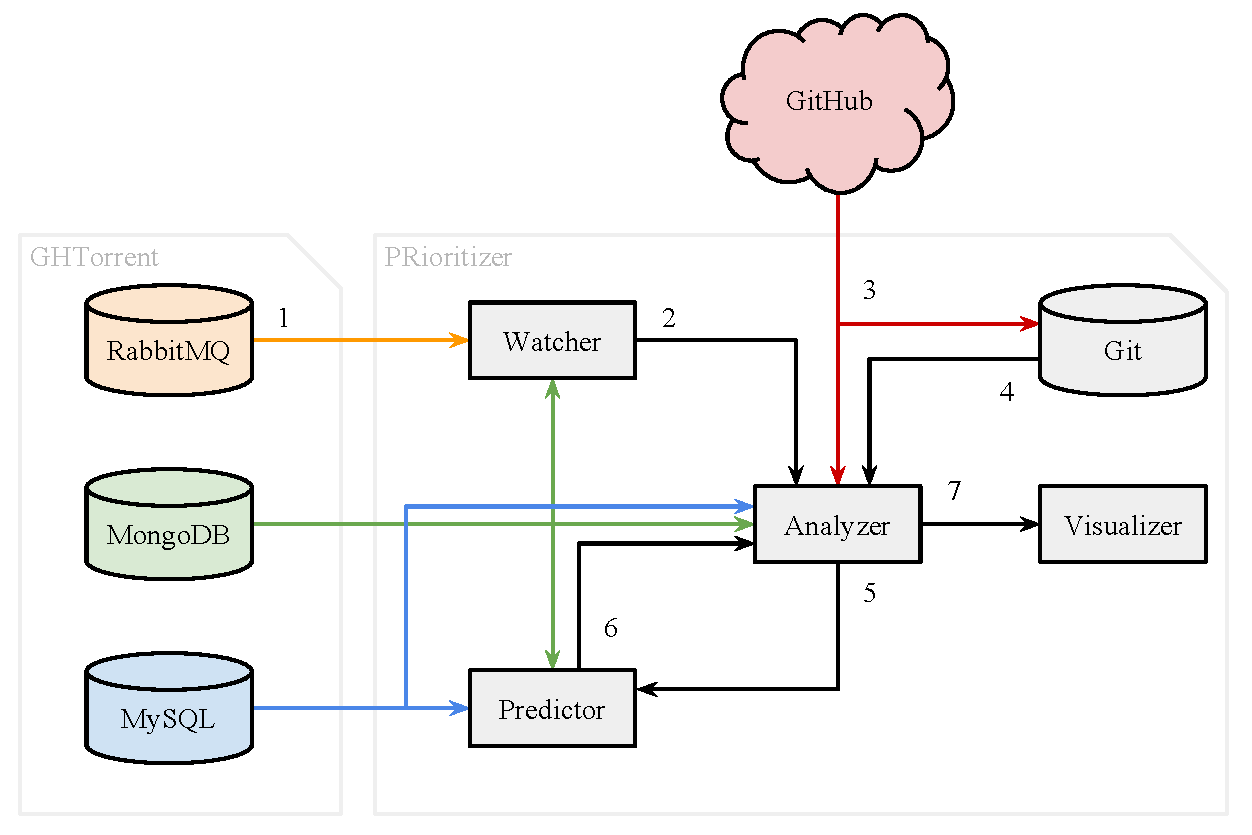
\includegraphics[width=0.5\textwidth]{../figs/architecture.pdf}
  \caption[Diagram of the architecture]
   {Diagram of the architecture. It shows the different data sources and components used by the \prioritizer service.}
  \label{fig:architecture}
\end{figure}

We designed \prioritizer as a loosely-coupled architecture based on independent
micro services. Figure~\ref{fig:architecture} shows a global overview of the
architecture.  The \prioritizer service uses two main data sources: GitHub and
the \ghtorrent project.  When an event arrives the \emph{watcher} component is
notified (1) and starts prioritizing the project (2).  When the \emph{analyzer}
gets a prioritization request it fetches a list of open pull requests from
GitHub and the pull request contents to the local Git clone (3).  When the data
is fetched, the analyzer processes each pull request in the list with data from the local
clone and \ghtorrent (4).  The data is now ready to be processed by the
\emph{predictor} (5), which generates an ordering for the pull requests.  After
the ordered list is returned to the analyzer (6), the output is generated and
available for the \emph{visualizer} (7).  Details about the design are presented 
in the following sections.

\paragraph{GHTorrent}
\ghtorrent~\cite{G13} mirrors all data exposed from the GitHub \api in
real time. It monitors the GitHub event timeline \api endpoint and publishes the 
retrieved data to a queue service (RabbitMQ) where multiple clients can connect to. 
It also maintains 2 databases, an unstructured one (MongoDB)
which contains the raw replies from the GitHub \api and a relational one
(MySQL) which stores indexed historical data for all GitHub repositories.
\prioritizer uses \ghtorrent as a source for both live and historical data. The live data
that the \prioritizer is interested in are events on pull requests triggered by actions 
such as assignment of the pull request to a specific user or merging the pull request.

\paragraph{Watcher}
The watcher listens to pull request event from \ghtorrent
via a RabbitMQ message queue. It maintains a list of registered repositories
and informs the analyzer when pull request events for one of those is
repositories is received.

\paragraph{Analyzer}
The analyzer analyzes pull request events and computes values for
the features presented in Section~\ref{sec:features}. To do so, for each repository,
it maintains a local Git checkout and a list of open pull requests.
On every pull request event, it updates both the Git repository with
a branch corresponding to the source branch of the pull request
and the open pull request list with fresh information from \ghtorrent.
Then, it uses both \ghtorrent and information into the raw pull request
data to calculate all features in the current time window.

The analyzer also implements a high-performance pairwise conflict detection
mechanism for branches that works by simulating pairwise merges in memory. To
avoid recomputing valid branch merges, it caches intermediate results.

To maintain high performance, all independent processes (Git repository
updating, conflict detection etc) are initiated asynchronously and their
results are gradually composed towards a final set of metrics for the processed
pull request.

\paragraph{Predictor}
The predictor calculates the probability that a specific pull request will
be active within the next time window. To do so, it maintains a per repository
model extracted by applying a machine learning algorithm to existing pull
requests and then uses the computed model to calculate probabilities for
currently updated pull requests.

The predictor is split in two parts: the historic data calculator and
the machine learning implementation. The first shares code (but not the
runtime) with the analyzer as both tools basically compute the same
values in different time windows. To capitalize on the wealth of available
options in statistical environments such as R, the machine learning
part is implemented as a different service that communicates with the
main predictor process through file exchange.

\paragraph{Visualizer}

The visualizer visualizes a list of pull requests, enriched with extra
information extracted from the analysis and prediction phases.  To address
reported deficiencies in GitHub's pull request user interface (also discovered
through our user survey), the visualizer supports filtering pull requests based
on specific branches, originating in specific authors, having conflicts or tests
and being in a mergable state.  It also supports sorting pull requests based on
a multitude of criteria, including all features reported in
Section~\ref{sec:features}.  A key feature of the visualizer is support for user
feedback on the prioritization; the user can report if the proposed
prioritization order is correct and change it to indicate what is the correct
one. \erik{Is this still true? Answer: I think it is not really a key feature,
but it could be in the future. Yes, the user is able to report a thumbs up/down,
but it is only collected yet, it doesn't feed the algorithm. }

The visualizer is implemented as a static web application; a
screenshot of its main page can be seen in Figure~\ref{fig:ui}.

\begin{figure}
  \centering
  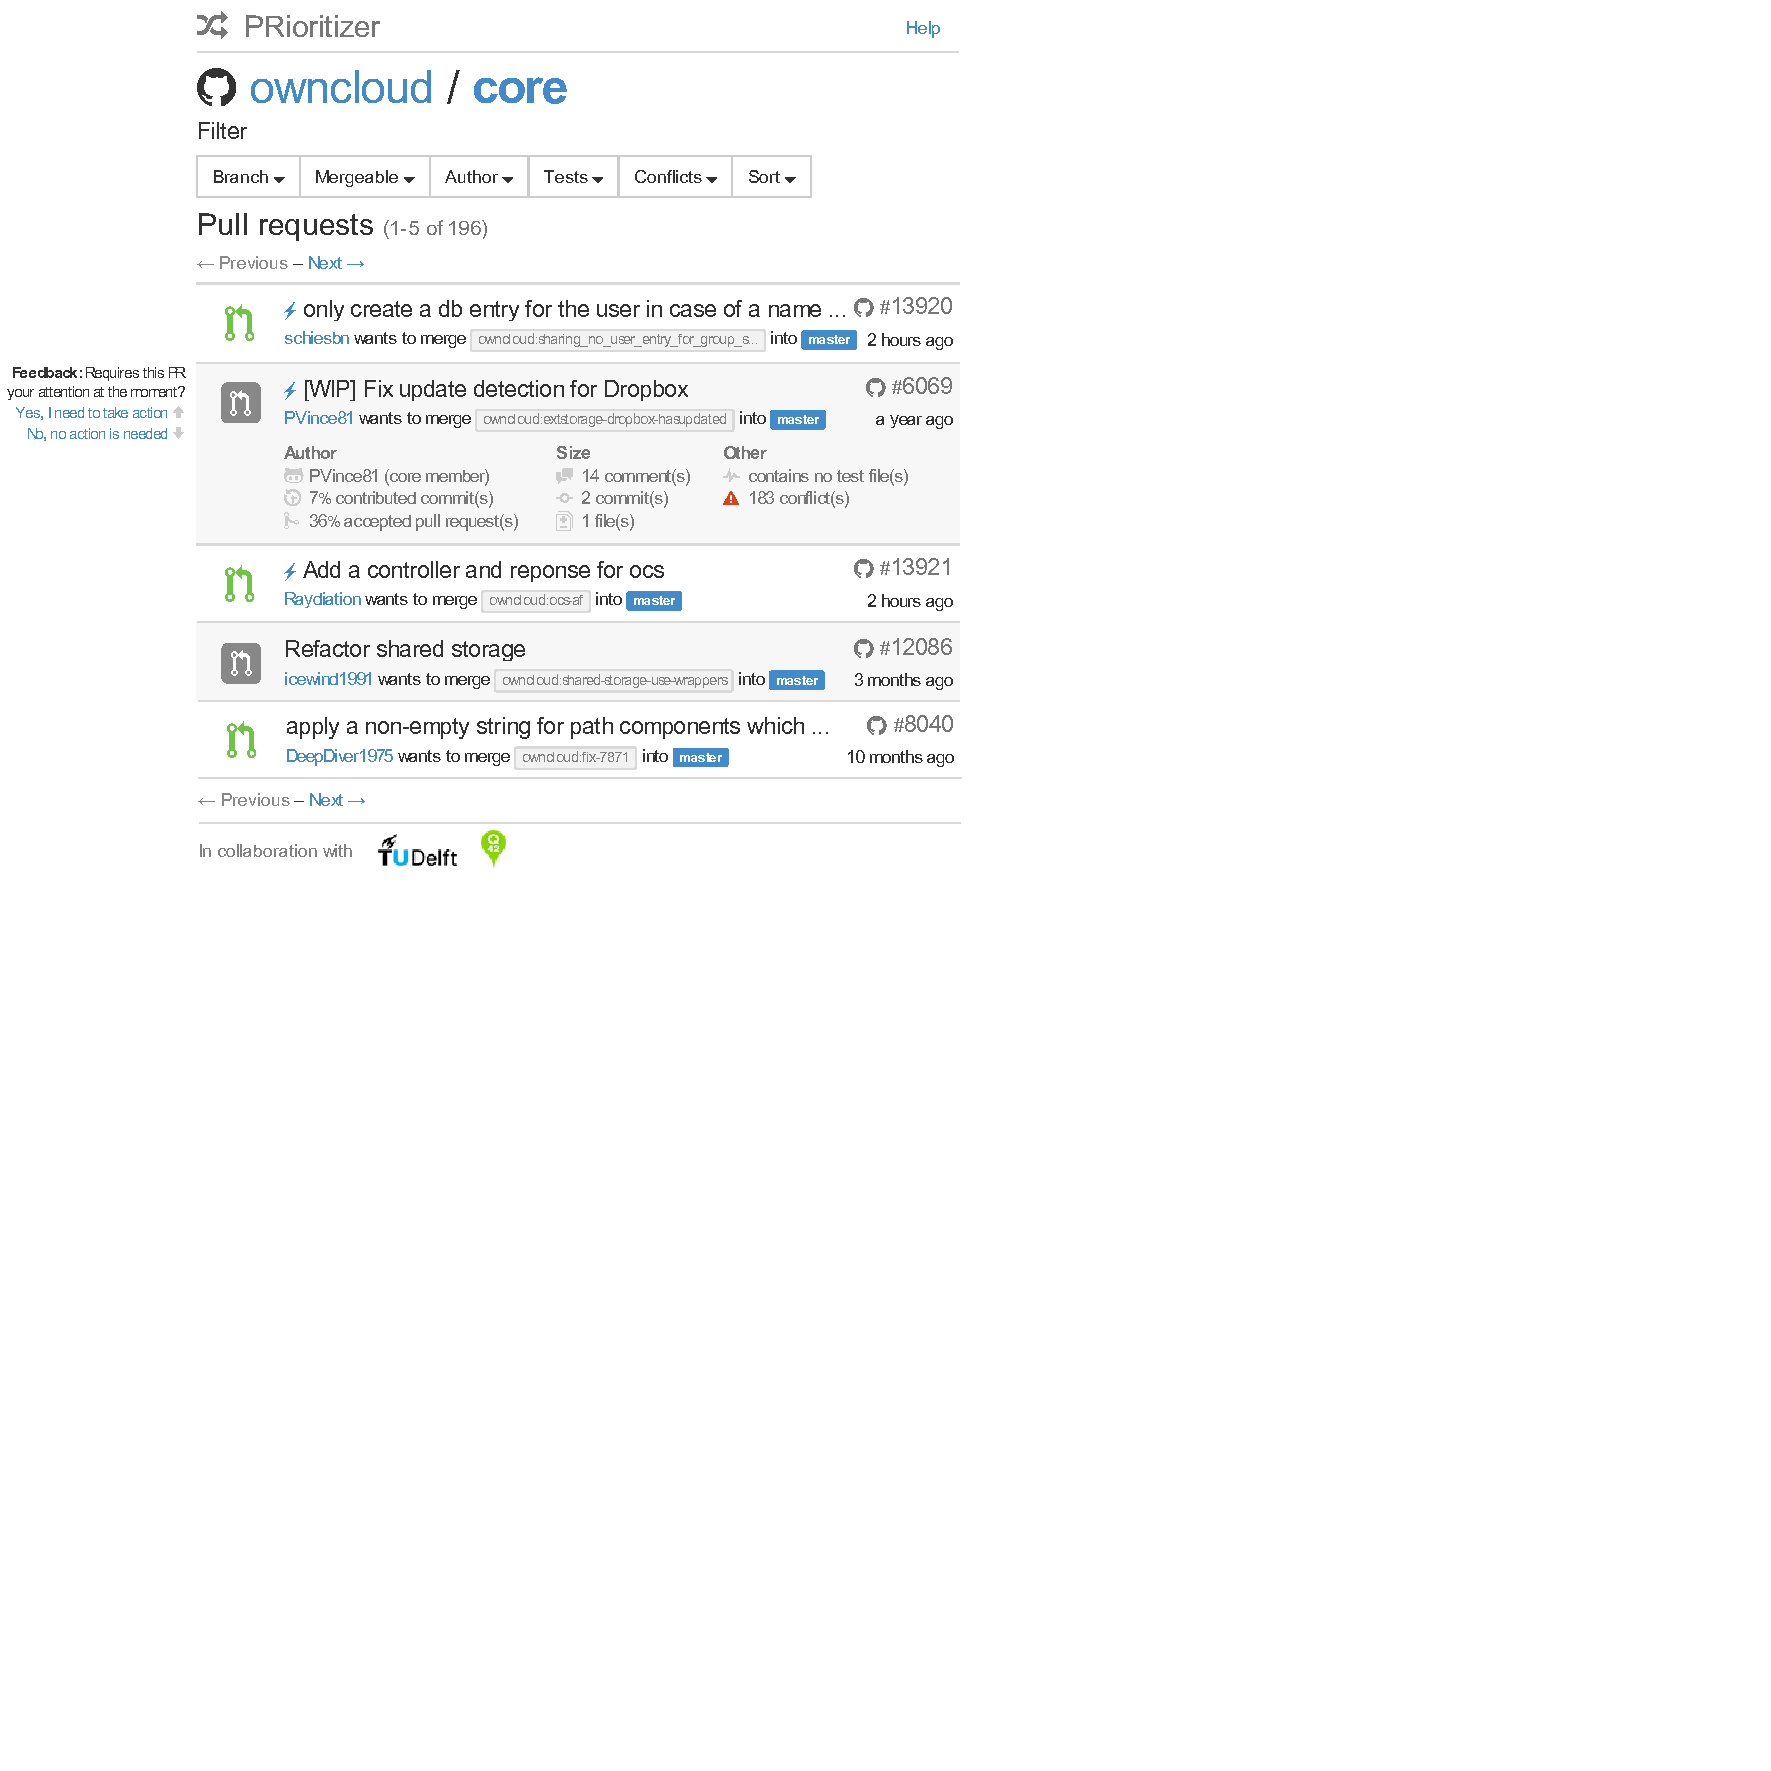
\includegraphics[width=0.5\textwidth]{../figs/interface.pdf}
  \caption[The user interface]
  {The user interface. It shows an ordered list of pull requests that need attention.}
  \label{fig:ui}
\end{figure}

\section{Initial Evaluation}
\label{sec:evaluation}

\subsection{How good are the activity predictions?}
\label{sec:learning}

To select one algorithm to base our prediction engine on, we used historical
data from 475 projects and three commonly used machine learning algorithms:
Logistic Regression, Na\"ive Bayes and Random Forests. The target of the test
was to compare how well models build with each algorithm could predict whether a
pull request would become active in the next time window against the ground
truth.  We ran the three algorithms against each project with a 10-fold random
selection cross-validation. The models were trained with 90\% training data and
10\% testing data.

The results show that both Logistic Regression and Na\"ive Bayes perform badly
on precision and accuracy, which were our top priorities.  On the other hand,
Random Forests perform well over all, even though the recall performance leaves
something to be desired. To improve the performance, we tried several
optimisations like dataset balancing and feature pruning to no avail.

%\begin{table}
%  \begin{tabular}{lrrrrc}
%    \hline
%    \textbf{Algorithm} & \textbf{5\%} & \textbf{Mean} & \textbf{StDev} & \textbf{95\%} & \textbf{Histogram} \\
%    \hline
%
%    \bf{Logistic Regression}\\
%    Area Under Curve & 0.71 & 0.81 & 0.06 & 0.91 & 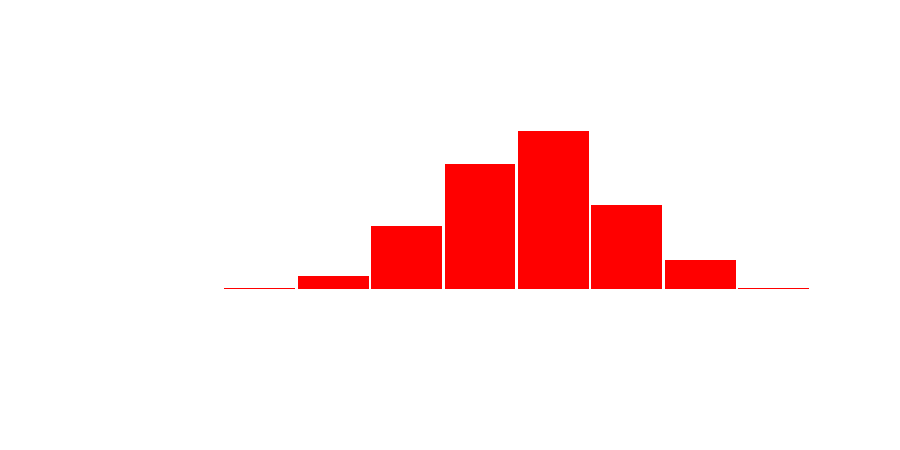
\includegraphics[scale = 0.1, clip = true, trim= 50px 60px 50px 60px]{../figs/hist-results/hist-LRauc.pdf} \\
%    Accuracy & 0.52 & 0.62 & 0.06 & 0.72 & 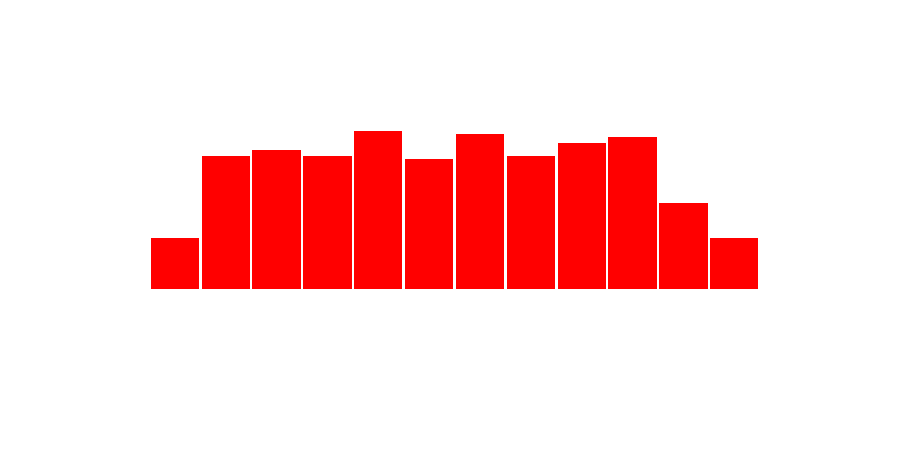
\includegraphics[scale = 0.1, clip = true, trim= 50px 60px 50px 60px]{../figs/hist-results/hist-LRacc.pdf} \\
%    Precision & 0.06 & 0.36 & 0.25 & 0.88 & 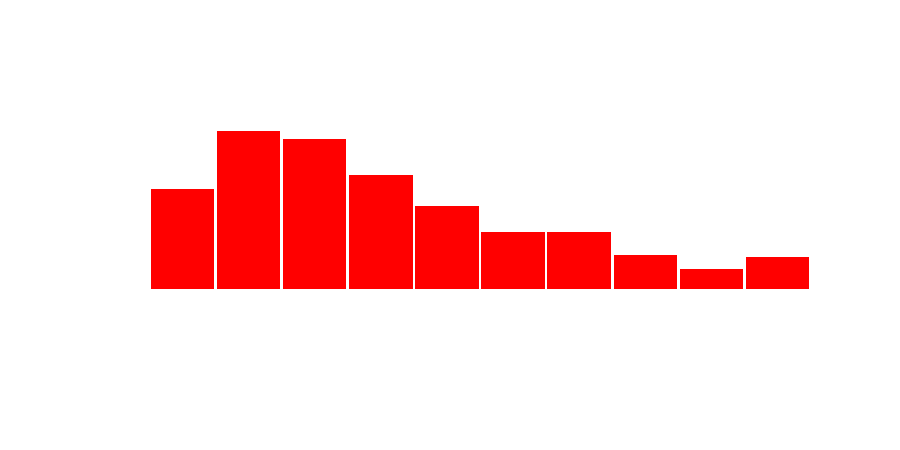
\includegraphics[scale = 0.1, clip = true, trim= 50px 60px 50px 60px]{../figs/hist-results/hist-LRprec.pdf} \\
%    Recall & 0.66 & 0.83 & 0.09 & 0.95 & 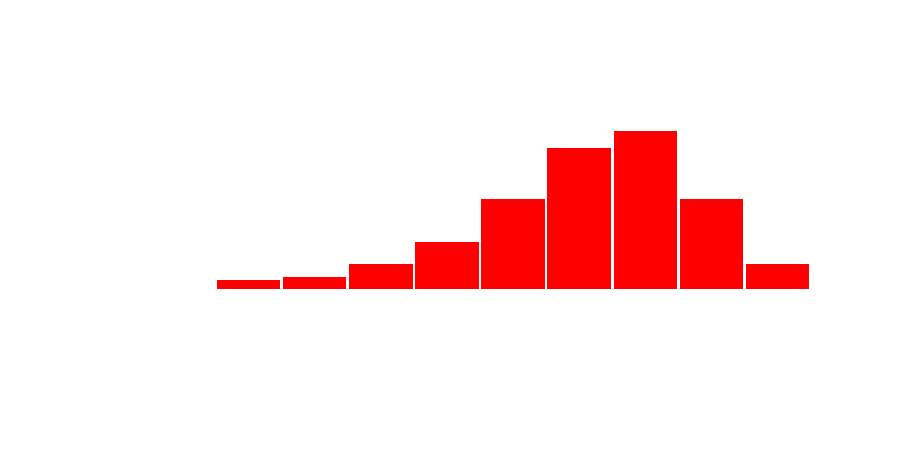
\includegraphics[scale = 0.1, clip = true, trim= 50px 60px 50px 60px]{../figs/hist-results/hist-LRrec.pdf} \\
%    F1 & 0.12 & 0.45 & 0.21 & 0.77 & 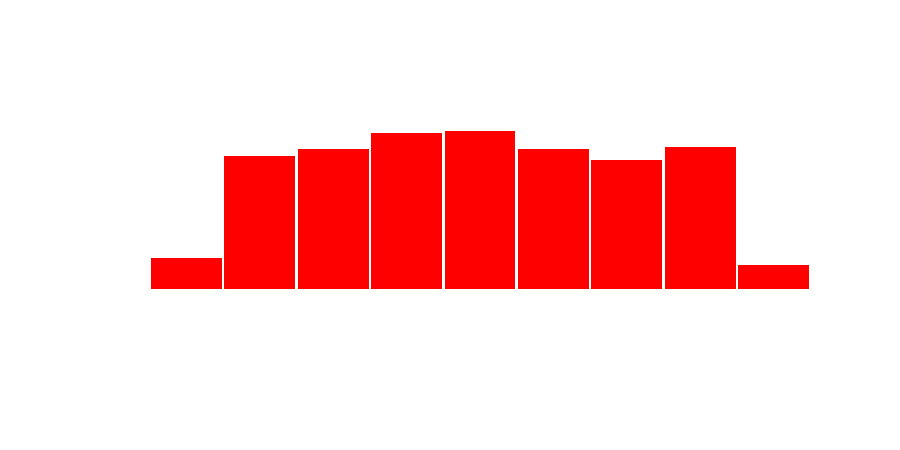
\includegraphics[scale = 0.1, clip = true, trim= 50px 60px 50px 60px]{../figs/hist-results/hist-LRf1.pdf} \\
%
%    \bf{Naive Bayes}\\
%    Area Under Curve & 0.65 & 0.75 & 0.06 & 0.86 & 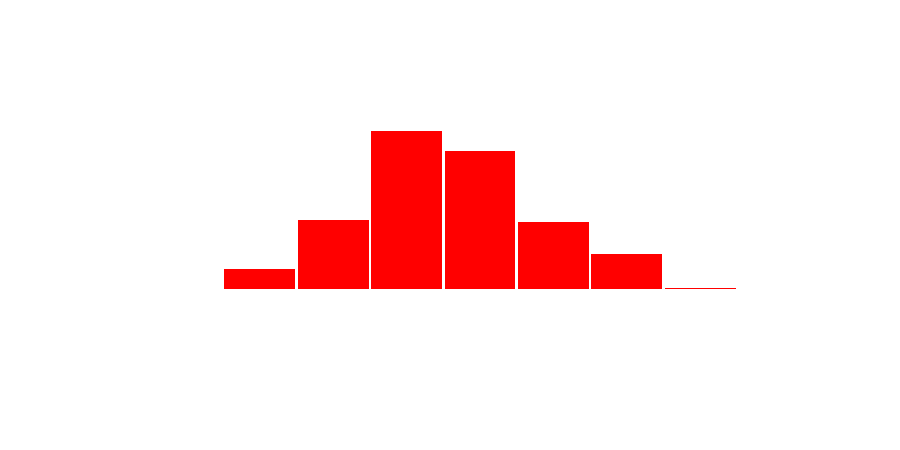
\includegraphics[scale = 0.1, clip = true, trim= 50px 60px 50px 60px]{../figs/hist-results/hist-NBauc.pdf} \\
%    Accuracy & 0.52 & 0.60 & 0.06 & 0.69 & 
\includegraphics[scale = 0.1, clip = true, trim= 50px 60px 50px 60px]{../figs/hist-results/hist-NBacc.pdf} \\
%    Precision & 0.06 & 0.34 & 0.23 & 0.82 & 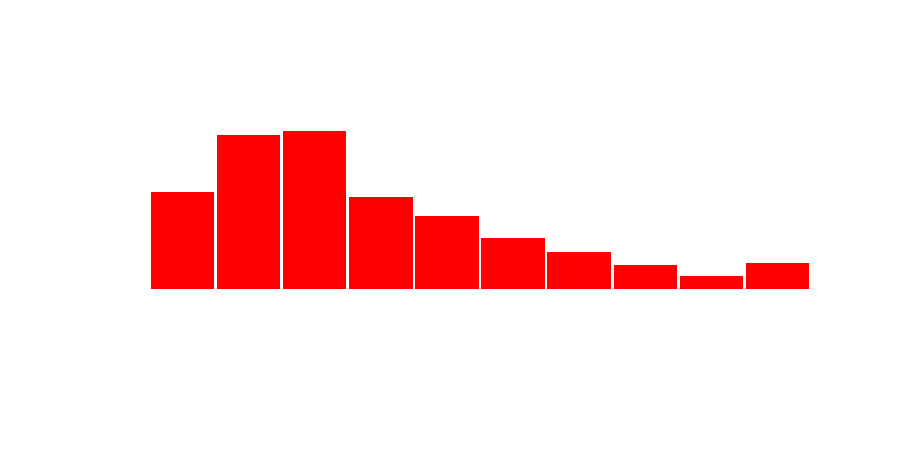
\includegraphics[scale = 0.1, clip = true, trim= 50px 60px 50px 60px]{../figs/hist-results/hist-NBprec.pdf} \\
%    Recall & 0.63 & 0.79 & 0.09 & 0.94 & 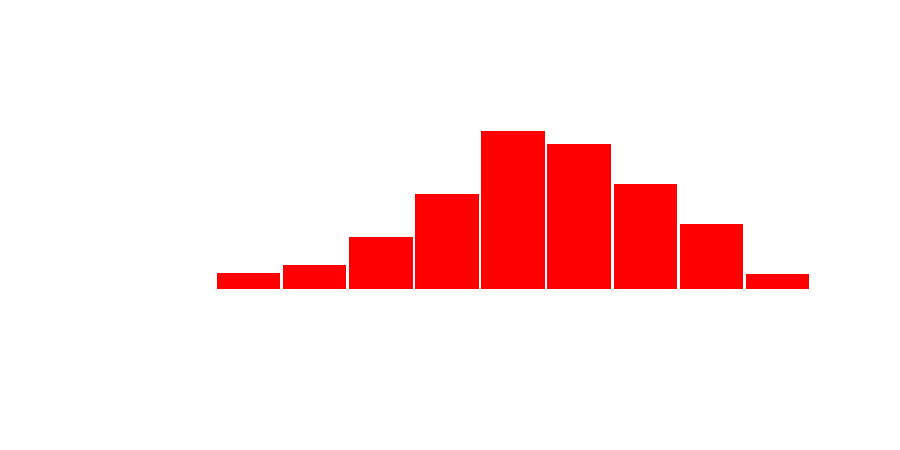
\includegraphics[scale = 0.1, clip = true, trim= 50px 60px 50px 60px]{../figs/hist-results/hist-NBrec.pdf} \\
%    F1 & 0.11 & 0.42 & 0.20 & 0.73 & 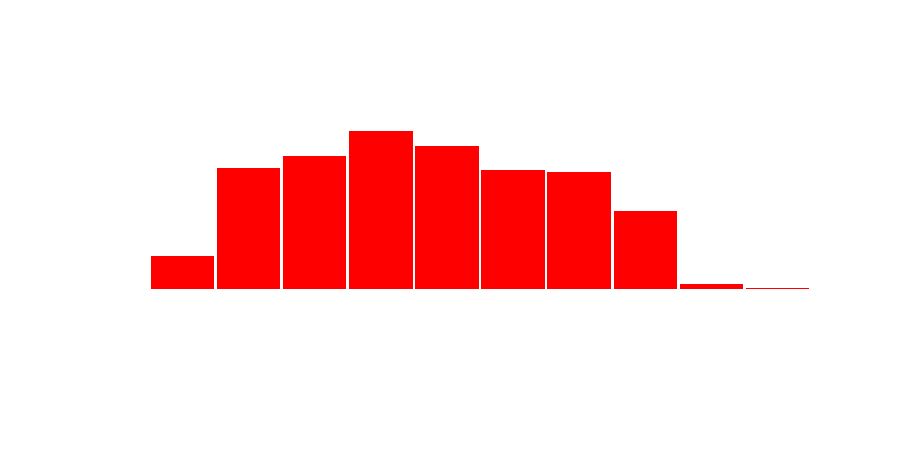
\includegraphics[scale = 0.1, clip = true, trim= 50px 60px 50px 60px]{../figs/hist-results/hist-NBf1.pdf} \\
%
%    \bf{Random Forest}\\
%    Area Under Curve & 0.81 & 0.89 & 0.05 & 0.95 & 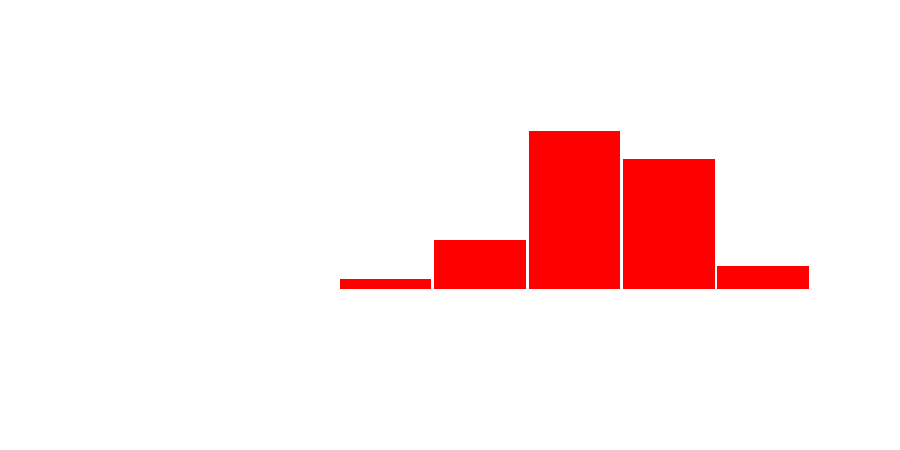
\includegraphics[scale = 0.1, clip = true, trim= 50px 60px 50px 60px]{../figs/hist-results/hist-RFauc.pdf} \\
%    Accuracy & 0.73 & 0.86 & 0.07 & 0.96 & 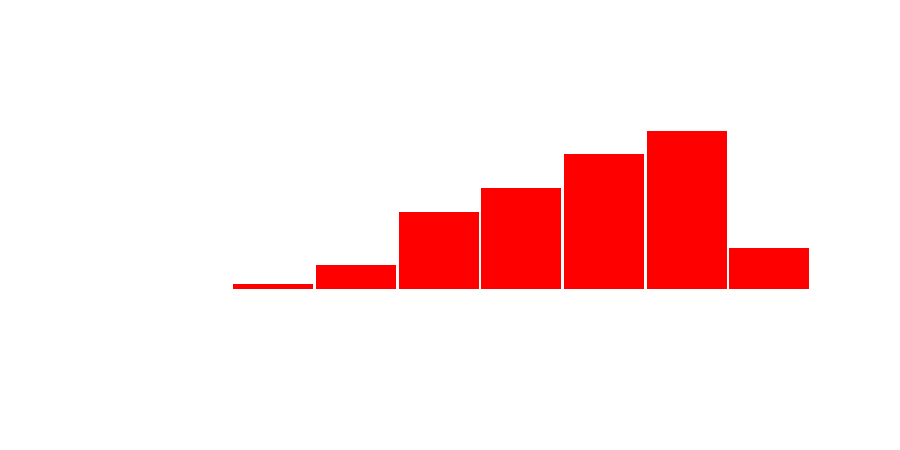
\includegraphics[scale = 0.1, clip = true, trim= 50px 60px 50px 60px]{../figs/hist-results/hist-RFacc.pdf} \\
%    Precision & 0.37 & 0.66 & 0.16 & 0.90 & 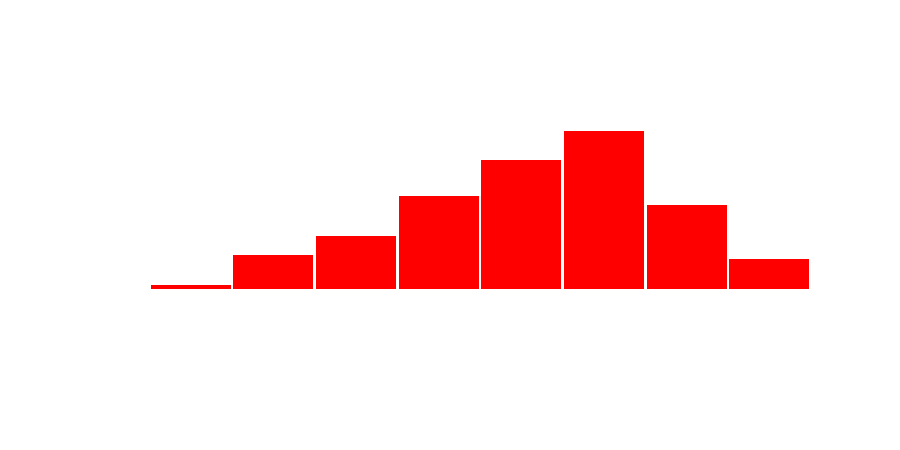
\includegraphics[scale = 0.1, clip = true, trim= 50px 60px 50px 60px]{../figs/hist-results/hist-RFprec.pdf} \\
%    Recall & 0.36 & 0.62 & 0.15 & 0.84 & 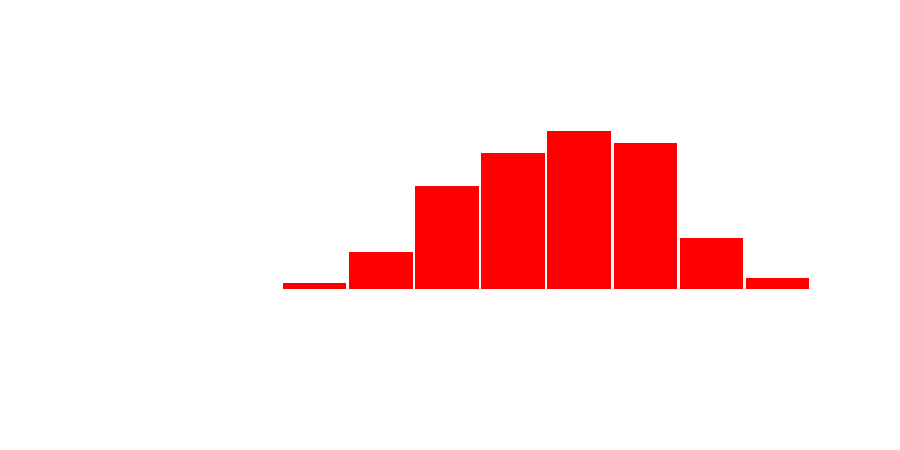
\includegraphics[scale = 0.1, clip = true, trim= 50px 60px 50px 60px]{../figs/hist-results/hist-RFrec.pdf} \\
%    F1 & 0.38 & 0.63 & 0.15 & 0.87 & 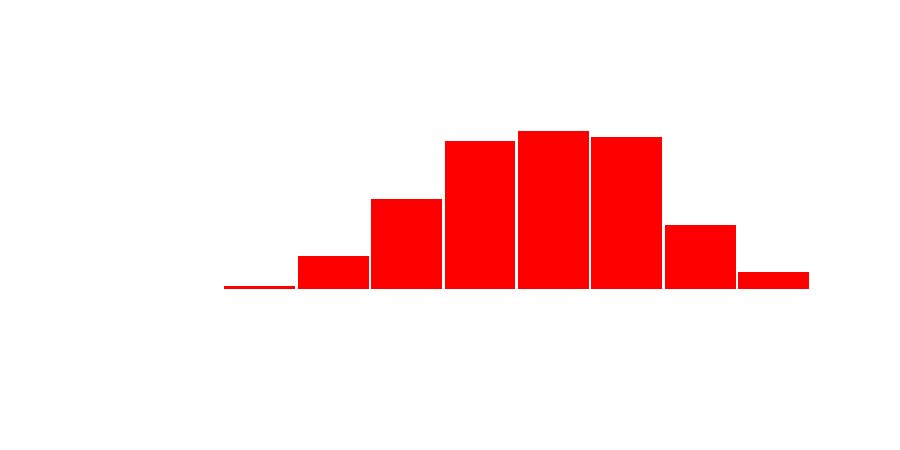
\includegraphics[scale = 0.1, clip = true, trim= 50px 60px 50px 60px]{../figs/hist-results/hist-RFf1.pdf} \\
%    \hline
%  \end{tabular}
%  \caption[Comparision of algorithms]{Scores and distributions of algorithm performance across projects.}
%  \label{tab:alg-compare}
%\end{table}

%It is interesting to see that the age is a very dominant factor when we look at
%the feature importance in figure~\ref{fig:feature-importance}.  This is probably
%the case because it is very likely that new pull requests receive comments
%within the first few days.  Since the age feature is so dominant it could impact
%the model in a bad way.  When we turned this particular feature off, the results
%were worse instead.  So it seems the age has a positive effect on the
%prediction.
%
%\begin{figure}
%  \centering
%  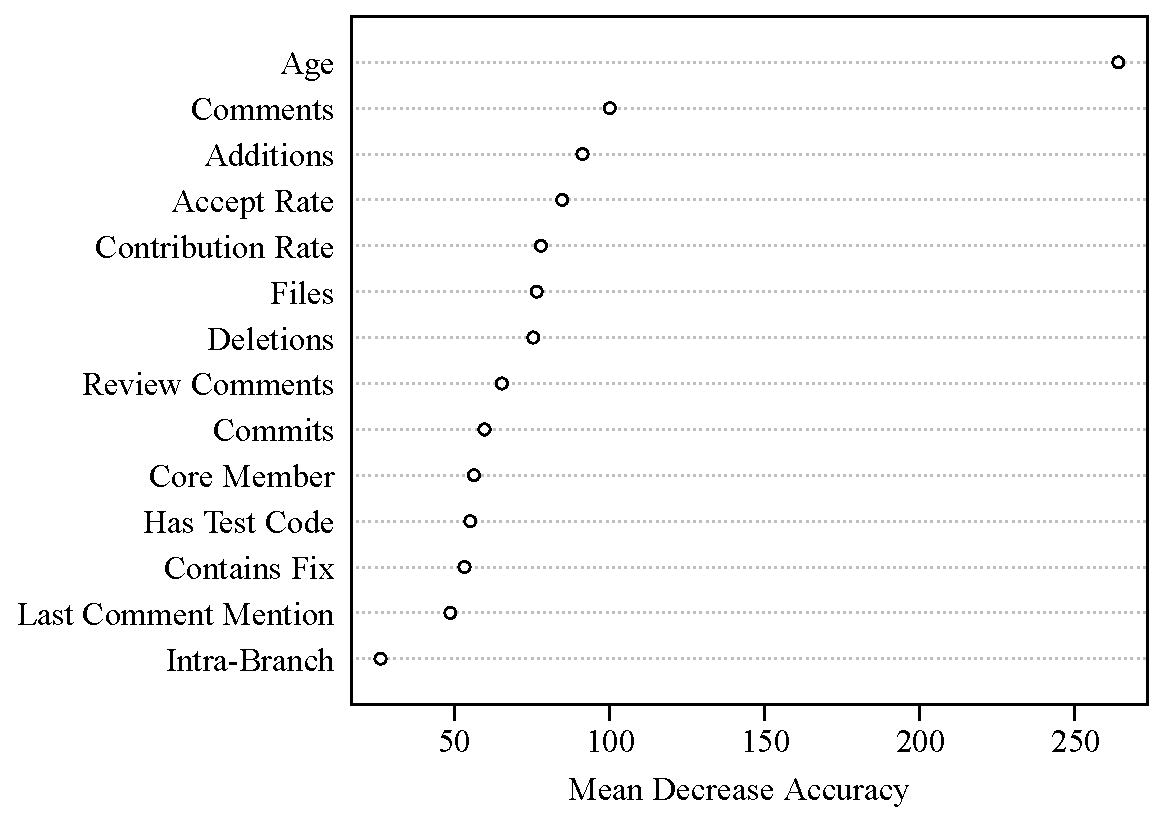
\includegraphics[width=0.45\textwidth]{../figs/mean-decrease-accuracy.pdf}
%  \caption[Plot of feature importance]
%   {Plot of feature importance of the aggregated projects. The age of the pull request is the dominant factor.}
%  \label{fig:feature-importance}
%\end{figure}

The results show that using Random Forests, we can predict with relatively
high accuracy (86\% on average) whether a pull request in a given time frame
of its life will be active in the next one. This is an important result
for building a prioritizer service, as it gives us the confidence to
recommend a default ordering to the service user. Moreover, as the
quality of the prediction varies across projects, we can build preprocessing
phases to determine whether default recommendations can be useful.
However, there is room for improvement: by selecting more representative
features, or custom features for each project, we can account for variations
of pull request handling practices. Moreover, user directed evaluation (already
implemented in the visualizer) can help retrofit our machine learning model
with user preferences.

\begin{figure*}[t]
\centering
\subfigure {
  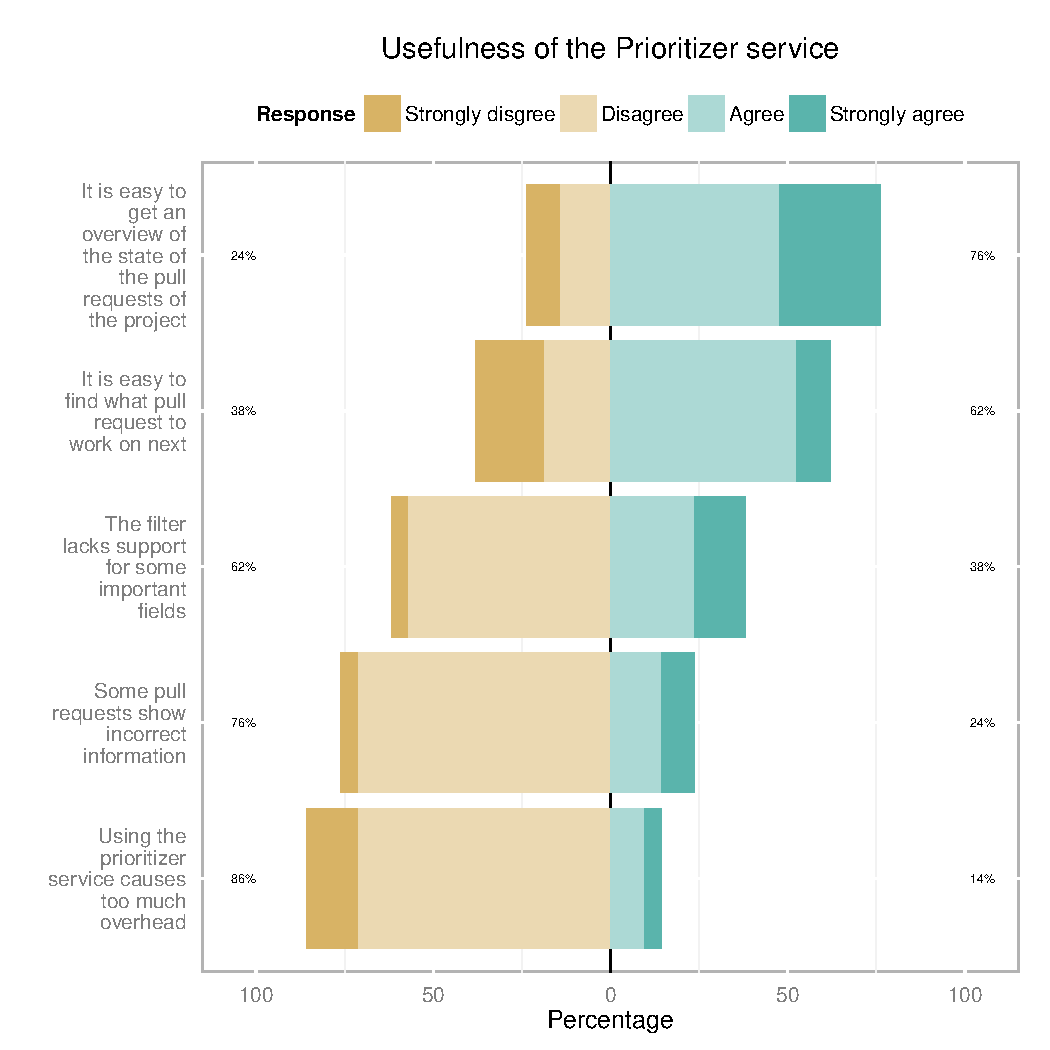
\includegraphics[scale=0.45]{service-userfulness}
  \label{fig:service-userfulness}
}
\subfigure{
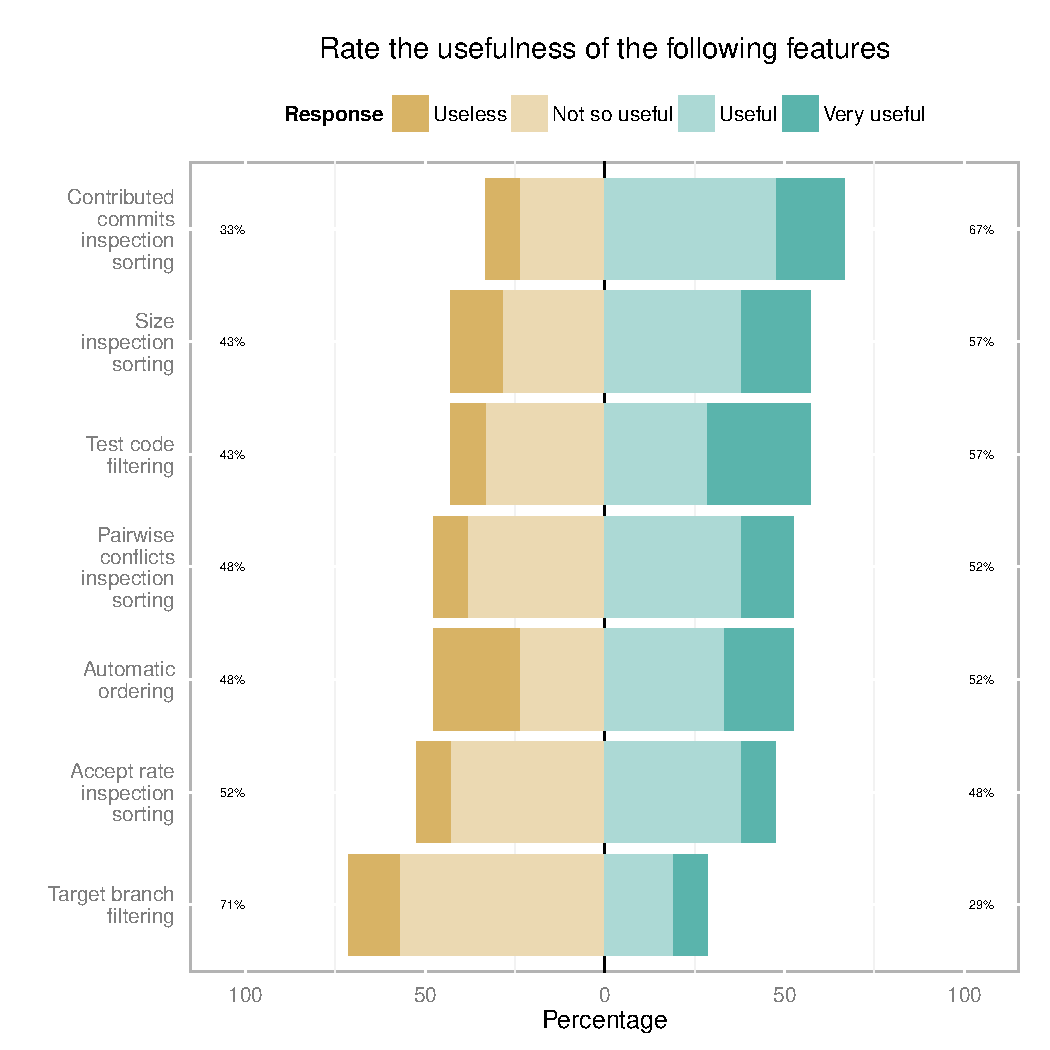
\includegraphics[scale=0.45]{feature-userfulness.pdf}
  \label{fig:service-userfulness}
}
\caption{User evaluation of the service and individual feature usefulness}
\label{fig:user-evaluation}
\end{figure*}

\subsection{Performance characteristics}

We hosted our service on a machine with a 3 GHz Xeon E5-1607 Quad 
core CPU and 16 GB of RAM. On average it is capable of prioritizing
6.7 PRs per second and performs 40 pairwise merges per second. In
practice it is around 400 pairwise merges per second due to the use of caching.
The whole process of prioritizing one repository, including updating the local Git clone, takes on average
1.1 minute. 

\andy{I would say the next paragraph can be dropped if we need space}
When multiple events for big repositories arrive at the same time, a single
\prioritizer instance processes them sequentially, which can cause a delay of a
few minutes. This can be solved by starting more watcher instances that
process events from the queue in parallel.

The \prioritizer runs incrementally on a set of pull requests. An initial import
with model training of a repository takes much longer than a normal run. Usually
it takes not more than a few minutes, but can take up to almost an hour
depending on the size of the project and of its pull requests.

\subsection{User Evaluation}

We performed a preliminary user evaluation in order to guide our future
developments of \prioritizer . For each of the 450 projects we used for
benchmarking, we invited core team members of those projects to use it.  The
invitation was by personal email containing a private link to the prioritizer
installation for their repository and a survey. The survey consisted of 4 odd
Likert-scale questions and 4 open ended ones. The Likert-scale questions invited
users to rate the usefulness of specific features and the overall service
quality while the open ended questions asked the users for missing features or
potential improvements. We received 21 answers.

Overall, as can be seen in Figure~\ref{fig:user-eval}, \prioritizer has been
positively perceived by human evaluators. The users seem to like that they
can easily obtain an overview of the overall state of pull requests in the
project. In the open ended responses, the users indicated that mergability
detection and contributor pull request profiling were their favourite
features.

\resp{5}{The fact you can see how much the author of the pull request did in the past and how his success rate for getting pull requests in.}

The main highlight of the service, the Automatic Ordering, received mixed
reviews;

is on average neither positive nor negative rated.
This has probably something to do with the reasons why a certain PR is ranked higher than others (\respnum{6,7,9,17,19,20}).
\resp{17}{It can show us the most pressing pull requests.
However, it is unclear how this ranking is established, so I'd hope to know why a pull request is considered more urgent then others.}


The next part is about the usability of the service.
Around 86\% (18) says that using the service causes no extra overhead.
The given answers have a correlation of $0.4441$ with the activity of the project.

76\% (16) of the respondents thinks the prioritized overview of PRs is clear enough.
\resp{1}{I can see at a glance which PRs can be merged automatically.
For some reason the Github PR interface does not show this, you have to click on a PR to find out if it can be automatically merged.
In one of my projects, PRs often sit unmerged for a while and have to be rebased, so it's better to know when rebasing is necessary sooner, rather than later.}

Only 62\% (13) of the respondents agree that the set of used and presented fields is complete.
It seems that the integrators of more active projects tend to disagree, with a correlation of $-0.4054$.
This probably caused by the fact that the prioritization service lacks support for GitHub labels and milestones.

Later on in the questionaire we asked to rate some features for a next version of the prioritization service.
71\% (15) of the respondents indicated that they want to prioritize according to labels.
The correlation between the activity and the lack of label support is $0.4443$.
\resp{7}{I like the autosorting, but I'd like more control over it.
I use labels a lot for things, so for example, `needs followup' is a label that means I need to take no action, so I'd love to be able to tell you that.}

As said earlier, it is not clear for everyone on what grounds one pull request is higher ranked than others.
Almost all respondents (86\% or 18) want more control over the automatic ordering in a future version.
\resp{19}{It's very difficult to tell what the default ordering means.
This might be an inevitable consequence of machine learning but without some insight into why the results were ordered in a certain way (and maybe the ability to tweak the input weights), the view wasn't helpful.}

Finally we asked the respondents if they would use the prioritization service for their project.
57\% (12) of the respondent gave a positive answer.
With a activity correlation of $0.4307$ it seems that integrators with a more active project tend to use it more than those with less active projects.
\resp{15}{I actually don't find it very useful at all.
I've never had a problem prioritising pull requests, we keep the number of open pull requests below 30.
Generally, I respond to all pull requests raised on the project as soon as I receive the notification for them.}

The results are not very conclusive.
It seems that in its current form the automatic ordering is not adequate.
Users want to see why a PR is considered more important than others and have more control over the learning process.
On the other hand the manual sorting and filtering options are positively evaluated.
The Pairwise Conflicts, Target Branch and Size are the most popular.
Although the latter two are fairly trivial features GitHub's interface doesn't support them.
This might be the reason why the are rated useful.
Finally, a narrow majority indicated that they will use the service for their project.

\section{Related Work}

\section{Conclusions and Future Work}

\section*{Acknowledgements} The authors would like to thank Audris Mockus for
fruitful discussions that influenced the design of the prioritization algorithm.

\bibliographystyle{IEEEtran}
\bibliography{prioritizer}


\end{document}
